% Column-width excerpt of the requant calibration file (schema, not a run).
\definecolor{tvink}{HTML}{111111}
\definecolor{tvmute}{HTML}{333333}

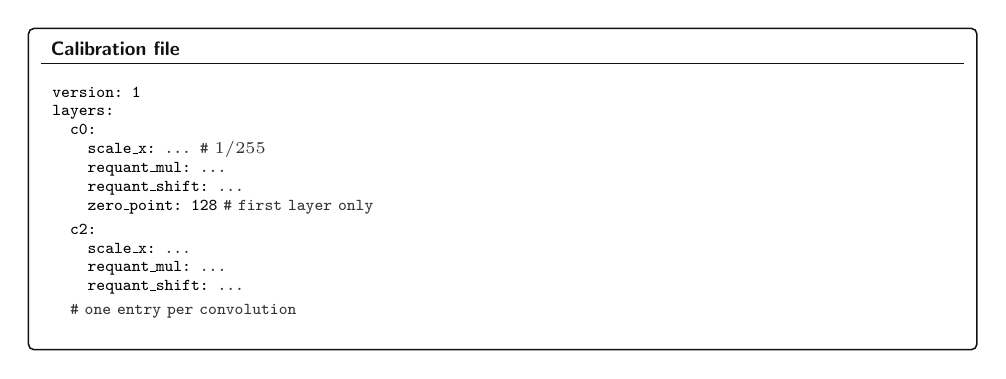
\begin{tikzpicture}[
  x=1mm, y=1mm,
  font=\sffamily\tiny,
]
\pgfmathsetmacro{\W}{\columnwidth/1mm - 0.8}

\draw[tvink, line width=0.55pt, rounded corners=2pt]
  (0, -0.8) rectangle (\W, 40.0);

\node[font=\sffamily\scriptsize\bfseries, text=tvink, anchor=west]
  at (1.6, 37.4) {Calibration file};
\draw[tvink, line width=0.4pt]
  (1.6, 35.5) -- (\W-1.6, 35.5);

\node[
  anchor=north west, align=left,
  font=\ttfamily\fontsize{5.6}{6.8}\selectfont,
  text width=0.90*\columnwidth
] at (1.8, 33.8) {%
version: 1\\
layers:\\
\quad c0:\\
\quad\quad scale\_x: \textcolor{tvmute}{\ldots}
  \textcolor{tvmute}{\# $1/255$}\\
\quad\quad requant\_mul: \textcolor{tvmute}{\ldots}\\
\quad\quad requant\_shift: \textcolor{tvmute}{\ldots}\\
\quad\quad zero\_point: 128
  \textcolor{tvmute}{\# first layer only}\\[0.3em]
\quad c2:\\
\quad\quad scale\_x: \textcolor{tvmute}{\ldots}\\
\quad\quad requant\_mul: \textcolor{tvmute}{\ldots}\\
\quad\quad requant\_shift: \textcolor{tvmute}{\ldots}\\[0.3em]
\quad \textcolor{tvmute}{\# one entry per convolution}%
};

\end{tikzpicture}
